\documentclass[11pt]{article}

\usepackage[margin=2.3cm]{geometry}
\usepackage{amsmath,amssymb,booktabs,array}
\usepackage{graphicx,xcolor,caption,enumitem,placeins}
\usepackage[hidelinks]{hyperref}
\usepackage{tikz}
\usetikzlibrary{arrows.meta,positioning}

\graphicspath{{figures/}{../figures/}}
\setlist[itemize]{topsep=3pt,itemsep=2pt,leftmargin=1.3em}
\setlist[enumerate]{topsep=3pt,itemsep=2pt,leftmargin=1.4em}
\captionsetup{font=small,labelfont=bf,skip=6pt}
\setlength{\parskip}{5pt}
\setlength{\parindent}{0pt}

\definecolor{navy}{HTML}{1F4E79}
\definecolor{rule}{HTML}{D0D5DD}

\pagestyle{plain}
\newcommand{\la}{list-aware}
\newcommand{\om}{off-market}

\title{\textcolor{navy}{Combined model development document}\\[4pt]
\large Both tracks, long version}
\author{List-aware and off-market}
\date{8 November 2026}

\begin{document}
\maketitle
\thispagestyle{empty}

\begin{center}
\small
\begin{tabular}{@{}>{\bfseries}l p{11.4cm}@{}}
Book & Synthetic Toronto sales, January 2021--May 2026, 150{,}000 closed sales \\
Claim window & December 2025--May 2026, 10{,}069 sales, walked forward one month at a time \\
List-aware & Walk-forward MdAPE \(4.28\%\), MAPE \(5.37\%\), median signed \(+0.90\%\) \\
Off-market & Walk-forward MdAPE \(7.45\%\), MAPE \(9.79\%\), median signed \(-0.37\%\) \\
Code & \texttt{features.py}, \texttt{models.py}, \texttt{run.py} \\
Track write-ups & Separate documents in \texttt{model-report/}, one for each track \\
\end{tabular}
\end{center}

\vspace{4pt}
{\color{rule}\hrule}
\vspace{8pt}

\section*{How to read this document}

This is the long version of the submission report. The four-page file the contest asks for will be cut from it after a proofread. The spine already follows that short report: the two questions, the shared data, the features, the two models and how we calibrate them, the walk-forward, the results, where each model fails, and the limits. The appendix holds the monitoring rules, the specifications we compared, and the references. The two track documents stay as the line-by-line specification. This one is the place the two models sit next to each other.

The numbers below are the ones \texttt{run.py validate} wrote for the adopted models. A home-level bootstrap around those pooled scores is in \texttt{reports/results\_table.tex}. We treat that interval as a lower bound, because homes sold in the same month share one market.

\tableofcontents
\newpage

\section{Summary}
\label{sec:summary}

We built two models because the contest asks two questions, and a model that sees the asking price is answering a different question from a model that has to find the price level itself. Mixing the two scores would make the off-market model look about three points tighter than it is.

\la{} predicts the close given the list price. On the six-month walk-forward its MdAPE is \(4.28\%\), against \(7.26\%\) for taking the ask as the forecast. The typical prediction is still about \(0.9\%\) high, in every month. \om{} predicts the sold price with no list price. Its walk-forward MdAPE is \(7.45\%\), against \(15.33\%\) for a 12-month community dollars-per-square-foot anchor. The pooled bias is about \(0.4\%\) low, and that pool hides a February that is \(4.4\%\) low.

Both models are one LightGBM, with the same tree settings, fit only on sales that have already closed. They share the size, lot, room, and location columns. They do not share a target, a text treatment, or a calibration. \la{} models \(\log(\text{sold}/\text{list})\) and multiplies back by the ask. \om{} models \(\log(\text{sold})\) and then applies one recent level shift. The place each one fails follows from that choice. \la{} is high on the cheapest homes and tight in the middle. \om{} is slightly high on the cheapest homes and about \(11\%\) low on the most expensive decile.

\section{Two questions, one book}
\label{sec:questions}

\begin{center}
\small
\begin{tabular}{p{3.2cm}p{5.6cm}p{5.6cm}}
\toprule
 & List-aware & Off-market \\
\midrule
Question & What will this listing close at? & What is this home worth before anyone has published an ask? \\
Who uses it & A desk that can see the listing. & A desk marking a home that is not yet listed. \\
Test file & \texttt{test\_list\_aware}, 4{,}064 homes, listed 1 Aug 2025--28 Sep 2026. & \texttt{test\_off\_market}, 3{,}974 homes, same window, no list price. \\
What we return & One dollar price, \(L\exp(\hat g)\). & One dollar price, \(\exp(F(x))\exp(-\delta)\). \\
What we do not return & An interval, a probability of selling over the ask, or a recommended haircut. & An interval, or a second correction the user is invited to change. \\
\bottomrule
\end{tabular}
\end{center}

The list price on the full book has correlation \(0.986\) with the sold price. That is why \la{} looks much tighter, and why \om{} is forbidden from using the column. The off-market test file does not have it. A model trained on it would be a list-aware model with the wrong name.

The handout weights the off-market track twice the list-aware track on the hidden test. We report the two errors separately for that reason. The published bars we have to clear, which we did not refit, are a simple type-and-neighbourhood 12-month median at \(17.7\%\) MdAPE / \(22.0\%\) MAPE, the starter ten-nearest-sales model at \(20.8\%\) / \(27.4\%\), and the list price itself at \(7.3\%\) / \(8.1\%\). Our own refit of the list price on these 10{,}069 sales is \(7.26\%\) / \(8.09\%\).

\section{Shared data}
\label{sec:data}

\subsection{Source and the split we both use}

The sales file is the same synthetic book. Names, streets, and coordinates do not line up with real maps, so we join nothing external. Outside data: none.

\begin{center}
\small
\begin{tabular}{lrrl}
\toprule
Sample & Rows & From & Through \\
\midrule
All closed sales & 150{,}000 & 1 Jan 2021 & 31 May 2026 \\
Developmental estimation & 139{,}931 & 1 Jan 2021 & 30 Nov 2025 \\
Developmental validation and walk-forward & 10{,}069 & 1 Dec 2025 & 31 May 2026 \\
Inner screen, both tracks & 9{,}886 & 1 Jul 2025 & 30 Nov 2025 \\
\bottomrule
\end{tabular}
\end{center}

The inner screen is where we chose windows, phrases, the building rule, the remarks score, and the off-market shift weight. The model for that screen was fit on sales through June 2025. Those months then go back into the developmental estimation sample. That reuse is why the walk-forward number, which never scores a month the tree has seen, is the claim we quote.

Six property types. On the estimation sample the shares are condo apartment \(51.1\%\), detached \(28.6\%\), semi-detached \(9.5\%\), condo townhouse \(6.8\%\), freehold townhouse \(3.4\%\), and co-op apartment \(0.5\%\). Five municipalities, 145 communities, 16 styles. Training sold-price median \(\$856{,}650\), mean \(\$1{,}073{,}917\), maximum \(\$30{,}000{,}000\).

\subsection{Fields we looked at and left out of both models}

\begin{center}
\small
\begin{tabular}{p{3.4cm}p{11.0cm}}
\toprule
Field & What we did \\
\midrule
Sold price, sale date & The target and the clock. \texttt{hide\_answers} strips both before a validation row is scored. \\
Days on market & Median 12 days. Known when the sale closes. Using it would leak the path from list date to sale date. \\
Third-party AVM & Filled on \(99.1\%\) of training sales and on no test row. The estimate date runs past the last training sale. \\
List price & An input to \la{} only. Correlation with sold price \(0.986\). Absent from the off-market test file, and stripped by \texttt{hide\_answers} on that track. \\
\bottomrule
\end{tabular}
\end{center}

\section{Shared preparation, then the fork}
\label{sec:clean}

We drop no sale. The first four steps are the same for both tracks. The fifth step is where the designs split.

\begin{enumerate}
\item Parse \texttt{house\_area}. A range \(a\)-\(b\) becomes the midpoint \(S=(a+b)/2\). A single number is the case \(b=a\). Both models then use \(\log S\). Skew of square feet falls from \(2.90\) to \(0.60\).
\item Encode the lot. Frontage and depth are missing together on \(58.2\%\) of training rows. Condo apartment, condo townhouse, and co-op are entirely missing. Detached, semi-detached, and freehold townhouse always have a lot. Filling the hole with a typical house frontage would invent land the unit does not have.
\item Leave bedrooms, washrooms, parking, and garage as recorded integers. Parking and garage can be zero, so a log is undefined. Latitude and longitude stay in degrees.
\item Add \(\sin(2\pi m/12)\) and \(\cos(2\pi m/12)\) of the listing month, so December sits next to January.
\item Build the track-specific columns from sales that have already closed. That construction is Section~\ref{sec:features}.
\end{enumerate}

The lot encoding, used by both:
\begin{align*}
\texttt{lot\_missing} &= \mathbf{1}\{\text{frontage is missing}\},\\
\texttt{log\_lot\_front} &= \log(\text{frontage})\ \text{when present, and}\ 0\ \text{when missing},\\
\texttt{lot\_depth} &= \text{the recorded depth, or}\ 0\ \text{when missing}.
\end{align*}
The zero on a missing frontage is \(\log 1\). Depth stays in feet: its skew is \(0.61\), and the log of depth has skew \(-0.38\).

\begin{center}
\small
\begin{tabular}{lrrl}
\toprule
Column & Skew & Skew of the log & What we did \\
\midrule
Sold price & 5.04 & 0.80 & Log. Inside the target of both models. \\
List price & 5.07 & 0.82 & Log feature, \la{} only. \\
Square feet & 2.90 & 0.60 & Log feature, both. \\
Lot front & 1.19 & 0.02 & Log, plus the missing flag, both. \\
Lot depth & 0.61 & \(-0.38\) & Feet, both. Zero if missing. \\
Washrooms, parking, garage & 1.2--1.7 & --- & Counts, both. \\
Bedrooms & 0.37 & --- & A count, both. \\
Latitude, longitude & 0.28, 0.37 & --- & Degrees, both. \\
\bottomrule
\end{tabular}
\end{center}

There is no winsorisation. The \(\$30\) million sale stays in. The log target, the median metric, and a minimum of 20 rows in a leaf are what keep that tail from setting the fit.

Two extra raw-field columns exist only on \la, because they describe the listing rather than a comp. One is frontage times depth, left missing when either side is missing. The other is 1 when the area was written as a range, so the tree can treat a midpoint as coarser. \om{} carries neither. It does build a building pin, latitude and longitude rounded to six decimals plus property type, and uses the pin only as a lookup key.

On \om, \texttt{lot\_missing} takes \(33\%\) of split gain. We read that as the house-versus-apartment cut, not as a land-value effect. On \la{} the same flag is \(0.07\%\) of gain, because the ask has already told the tree which product it is pricing.

\section{What the market looks like}
\label{sec:market}

The price level is not a fixed mean, and the two models spend their complexity in different places because of that.

On the monthly median sold price, an augmented Dickey--Fuller test with a trend gives \(p = 0.033\), and a KPSS test with a trend does not reject stationarity around that trend (statistic \(0.093\), below the \(10\%\) critical value \(0.119\)). A robust STL split gives seasonal strength \(0.80\): May high, January low, a swing of about \(\$144{,}000\) around the trend. That swing is why both models carry the listing-month sine and cosine. It is a small share of gain once a recent price is in the design, which fits the idea that the comps already carry the level.

\begin{figure}[ht]
\centering
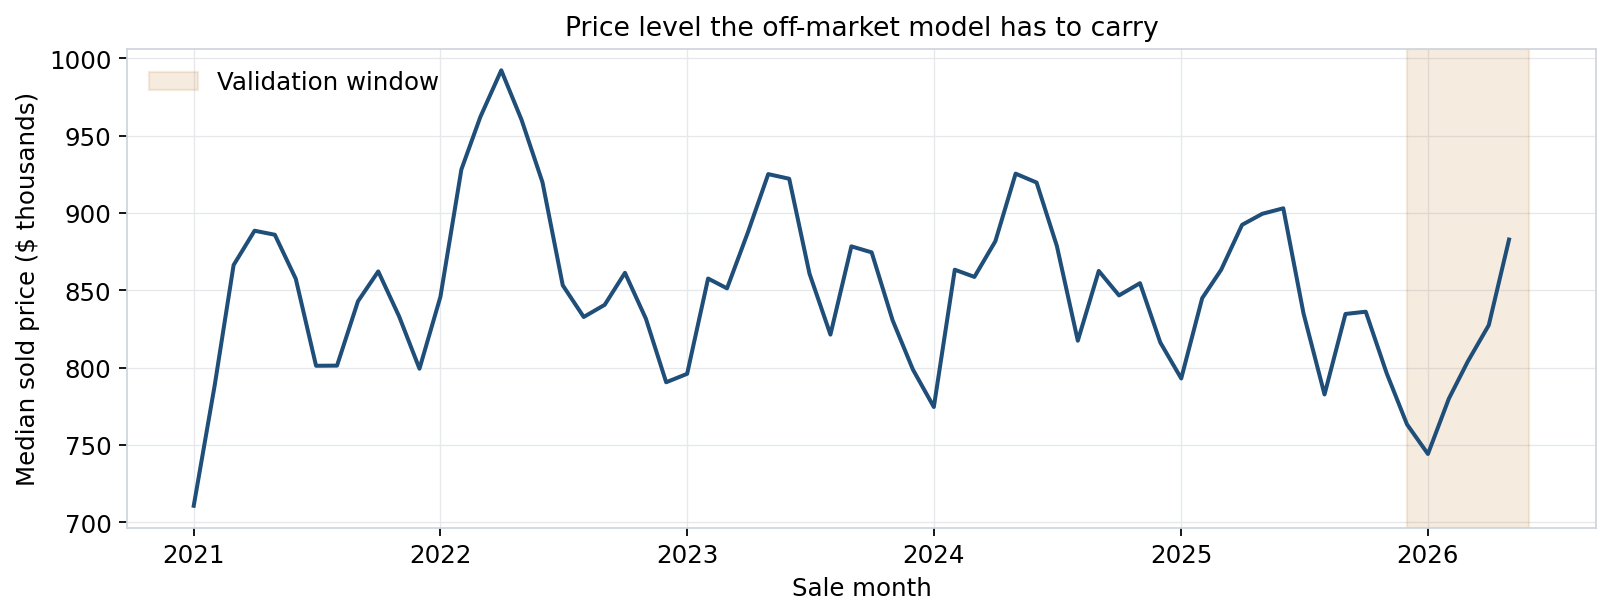
\includegraphics[width=\linewidth]{om_monthly_price.png}
\caption{Median sold price by month. The band is the validation window. Both models have to live with this path. Only \la{} also sees the ask.}
\label{fig:monthly}
\end{figure}

The ask is a strong quote and a moving one. Over the full book the median sold-to-list ratio is \(0.98\), so the typical home closes \(2\%\) under the ask. In the validation window the list-price forecast sits \(5.68\%\) above the sold price. A constant historical discount would be the wrong size for late 2025 and early 2026.

\begin{center}
\small
\begin{tabular}{p{4.2cm}p{5.2cm}p{5.2cm}}
\toprule
Fact & What \la{} does with it & What \om{} does with it \\
\midrule
The ask already holds the level & The target is the log gap around the ask. Attributes explain the miss. & The ask is unavailable. The tree has to produce the level. \\
The gap drifts & A SARIMAX residual forecast enters as \texttt{list\_month\_factor}, plus a one-month city lag and a three-month local discount. & A single shift \(\delta\), re-estimated from the three months before the origin. \\
Seasonality is in the price level & The sine and cosine are a small control. The ask already contains most of the season. & The same pair, plus 3-month and 12-month city dollars per square foot. \\
A log-linear fit on attributes & \(R^2 = 0.966\) once \(\log L\) is in. Elasticity on the ask \(0.894\). & \(R^2 = 0.713\), square-foot elasticity \(0.496\). Developmental MdAPE \(20.3\%\), behind the community anchor. \\
\bottomrule
\end{tabular}
\end{center}

The list-aware time-series piece is worth stating once, because it is the reason \la{} has no second-stage shift. On the developmental sample we fit
\[
\log Y_i = \beta_0 + \beta_L \log L_i + z_i^\top\gamma + e_i
\]
and model the monthly mean residual. An augmented Dickey--Fuller test with a trend gives \(p = 0.0002\), so we do not difference. The fitted model on the 59 estimation months is a constant, a one-month autoregression, and a 12-month autoregression: intercept \(-0.0046\), AR(1) \(0.872\), seasonal AR(12) \(0.370\). In-sample \(R^2\) on the monthly series is \(0.885\). Adding that forecast back onto the log-linear prediction cuts developmental MdAPE from \(7.13\%\) to \(4.78\%\) and median signed error from \(+5.95\%\) to \(+0.25\%\). \la{} does not add the forecast on at the end. It passes the same number in as a feature and lets the tree decide how much to use.

\section{Features}
\label{sec:features}

\la{} has 23 columns. \om{} has 35. Twelve of them are the same cleaned attributes. The rest are the reason the models are different. Nothing in either design is the home's own sold price, a later sale, or a statistic computed on the unlabelled test file. Category levels are the values seen in the sales the model was fit on. An unseen level is missing, and LightGBM keeps the missing value.

\subsection{Which column is in which model}

\begin{center}
\small
\begin{tabular}{p{4.6cm}ccc}
\toprule
Column & Both & \la{} only & \om{} only \\
\midrule
\(\log S\), lot flag, log frontage, depth & \(\bullet\) & & \\
Beds, baths, parking, garage, lat, lon & \(\bullet\) & & \\
Listing-month sine and cosine & \(\bullet\) & & \\
Type, style, municipality, community & \(\bullet\) & & \\
\(\log L\) & & \(\bullet\) & \\
\texttt{lot\_area}, \texttt{area\_is\_range} & & \(\bullet\) & \\
\texttt{peer\_ask} & & \(\bullet\) & \\
\texttt{recent\_discount} & & \(\bullet\) & \\
\texttt{market\_lag} & & \(\bullet\) & \\
\texttt{list\_month\_factor} & & \(\bullet\) & \\
\texttt{log\_community\_psf} & & & \(\bullet\) \\
\texttt{log\_city\_psf\_3}, \texttt{log\_city\_psf\_12} & & & \(\bullet\) \\
\texttt{building\_sales}, \texttt{building\_log\_price} & & & \(\bullet\) \\
13 phrase flags & & & \(\bullet\) \\
\texttt{remarks\_score} & & & \(\bullet\) \\
\bottomrule
\end{tabular}
\end{center}

Remarks were tried on \la{} as 20 singular vectors of a TF--IDF, fit on training text only. Developmental MdAPE moved from \(4.83\%\) to \(4.85\%\). We left the text out of \la. On \om{} the same source is a set of flags plus one ridge score, and the July--November screen kept both. The gain chart then shows the score is not the engine. We keep it because the screen that was not allowed to see December kept it.

\subsection{List-aware columns}

Peer ask is whether this ask, per square foot, is rich or cheap against homes like it that have already sold.
\[
\texttt{peer\_ask}_i = \frac{L_i/S_i}{m_{c(i),t(i)}(\tau_i)}.
\]
\(m\) is the median sold dollars per square foot in the same community and type, using sales that closed strictly before the listing month. Fewer than 30 sales falls back to the type. On the developmental validation rows the community cell is used for \(97\%\) of homes. This column is \(21.6\%\) of split gain, the largest share in \la.

The recent discount is the median of \(Y/L\) for the same community and type over the three sale months before the listing month, with the same floor of 30, then the type, then missing. Coverage is thin. On the developmental validation rows the community cell is used for \(15\%\), the type fallback for \(39\%\), and \(46\%\) are missing. Under walk-forward the window slides forward every month, which is one reason the walk-forward bias (\(+0.90\%\)) is smaller than the one-origin bias (\(+1.49\%\)).

\texttt{market\_lag} is the median of \(\log(Y/L)\) in the calendar month before the listing month, held flat past the last estimation month. \texttt{list\_month\_factor} is the SARIMAX forecast when the listing month is in the horizon, and the realized mean log residual of the previous month otherwise. The median value on the developmental validation rows is \(-0.0539\), about \(5.2\%\) below the log-linear fit. The three time columns all survive in the gain ranking, so we kept all three.

\subsection{Off-market columns}

Without an ask, the local tape has to be a price, not a ratio. For a home listed in month \(\tau_i\), with window \(W=12\),
\[
q^{\mathrm{comm}}_i = \operatorname{median}\{Y_j/S_j : \text{same community and type},\ \tau_i-W \le m_j < \tau_i\}.
\]
Fewer than 30 sales falls back to the type, then to the city, then to the median of every usable sale in the sample the table was built on. The column is \(\log q_i\). On the developmental validation rows the community cell itself is used for \(76\%\) of homes. Two citywide companions use the same construction over 3 months and over 12, with no community split.

We froze \(W=12\) on July--November. On that slice the 12-month anchor had MdAPE \(15.33\), the 6-month \(16.19\), the 24-month \(15.70\), and the full history \(16.42\) with signed error \(+11.97\%\). A blend that weights the community by \(n/(n+\text{strength})\) lost to the hard threshold of 30.

The building price is a second tape, for this building rather than this neighbourhood. A comp has the same pin, a sold date strictly before \texttt{date\_listed}, and a different listing number. Each historical dollars-per-square-foot is reindexed to the listing month with a type index that itself uses only earlier months,
\[
I_{t,m} = \operatorname{median}(\ell_{t,m-1},\ell_{t,m-2},\ell_{t,m-3}),
\]
where \(\ell_{t,m}\) is that type's median log dollars per square foot in month \(m\), forward-filled through empty months. If there is at least one eligible comp,
\[
\texttt{building\_log\_price}_i = \log\bigl(S_i \times \exp(I_{t,\tau_i})\times\operatorname{median}\{f_j\}\bigr),
\]
and \texttt{building\_sales} is the count. Otherwise the log price is missing and the count is 0. The gate is one prior sale. Requiring three, or adding the last sale and a repeat-sale of the same beds, baths, and area string, was worse on July--November. On the developmental validation rows, \(59.8\%\) of homes have at least one eligible earlier sale.

The phrase flags are 1 when the lower-cased remarks match a pattern we wrote down: as-is, turnkey, potential, original, finished, renovated, needs work, stunning or beautiful, and the five we added later (investor, motivated, redone, dated, worn). The extra five cut the predecessor's July--November MdAPE from \(8.41\) to \(8.33\). Each flag is under \(0.5\%\) of gain on the final tree.

The remarks score is a ridge of log sold price on a TF--IDF of unigrams and bigrams, penalty \(0.3\), at most 3{,}000 terms, minimum document frequency 40. Before the vectorizer runs we replace numbers with \texttt{NUM} and community names of four or more characters with \texttt{COMMUNITY}, so the score cannot memorise a printed price or a neighbourhood. Inside the estimation sample each row is scored from sales that closed earlier, in blocks at \(40\%\), \(55\%\), \(70\%\), \(85\%\), and \(100\%\) of the ordered sample. A home we are scoring gets the ridge fit on the whole past. July--November preferred the score by \(0.05\) MdAPE (\(7.97\) against \(8.02\)), both with the level shift on.

\subsection{What each tree actually splits on}

\begin{center}
\small
\begin{tabular}{lr@{\hspace{1.6em}}lr}
\toprule
\la{} feature & Gain & \om{} feature & Gain \\
\midrule
peer ask & 21.6\% & lot missing & 33.3\% \\
community & 18.6\% & building log price & 17.8\% \\
log list price & 9.6\% & log square feet & 12.9\% \\
market lag & 9.4\% & community & 12.4\% \\
recent discount & 7.5\% & log lot front & 8.3\% \\
list-month factor & 6.3\% & washrooms & 5.3\% \\
log square feet & 3.2\% & lot depth & 3.0\% \\
 & & log community \$/sqft & 2.0\% \\
 & & remarks score & 0.7\% \\
\bottomrule
\end{tabular}
\end{center}

Gain describes the fitted tree. It is not a causal ranking. Municipality is about \(0\%\) of gain in both models once community is present. On \la, the lot-missing flag is \(0.07\%\). On \om, property type is \(0.6\%\), because the lot flag has already made the house-versus-apartment cut.

\subsection{Candidates we tested and did not keep}

\begin{center}
\small
\begin{tabular}{p{2.2cm}p{4.6cm}p{7.4cm}}
\toprule
Track & Candidate & What happened \\
\midrule
\la & Remarks, 20 SVD components & Developmental MdAPE \(4.85\) against \(4.83\). \\
\la & Cumulative type-level sold-to-list median & Outer-window MdAPE \(4.63\) against \(4.53\). The three-month discount is a different feature and stayed. \\
\la & Rotated coordinates, clusters, 10 nearest sales & Developmental MdAPE \(4.52\)--\(4.53\). No improvement. \\
\la & A level shift on top of the month factor & Developmental MdAPE \(4.40\), the best one-origin cell. Walk-forward signed error \(-1.75\) on the related haircut. We did not adopt it. \\
\om & Predict the gap around the community anchor & Best walk-forward MdAPE \(7.50\), against \(7.45\) for the direct model. The gap model stays the challenger. \\
\om & Blend community and type medians & July--November preferred the hard threshold of 30. \\
\om & Three prior sales, last sale, repeat sale & Worse than one prior sale on July--November. \\
\om & Separate house and condo shifts & July--November \(8.18\) against \(8.17\) for one shift, on the gap model. \\
\om & A 75/25 blend of direct and gap & Tied the pure direct model. We kept the pure model. \\
\om & Quantile loss at the median & Walk-forward MdAPE \(7.53\), behind squared error. \\
\om & A land term and a drifting city forecast & July--November turned both off, so those predictions are the gap model's. \\
\bottomrule
\end{tabular}
\end{center}

\section{Calibration}
\label{sec:calibration}

Both models use the same tree. They do not use the same correction, because only one of them is missing the ask.

\begin{center}
\small
\begin{tabular}{p{3.4cm}p{5.7cm}p{5.5cm}}
\toprule
 & \la & \om \\
\midrule
Target & \(\log(Y/L)\) & \(\log Y\) \\
Loss & Squared error on the log gap & Squared error on log price \\
Reconstruction & \(\hat Y = L\exp(\hat g)\) & \(\hat Y = \exp(F(x))\exp(-w\delta)\), \(w=1\) \\
Second stage & None. The ask is the level, and the month factor is a feature. & One median log miss, from the three months before the origin, fit on a tree that did not see those months. \\
Settings & 127 leaves, learning rate \(0.03\), 700 trees, at least 20 rows in a leaf, row and column subsamples \(0.8\), L2 penalty \(1\), seed \(0\). & The same settings. We did not rerun the grid. \\
Categoricals & Type, style, municipality, community. & The same four. \\
Developmental shift & --- & \(\delta = +1.58\%\) on Sep--Nov 2025. Every Dec--May prediction is multiplied by about \(0.984\). \\
\bottomrule
\end{tabular}
\end{center}

Squared log error is a smooth proxy for percentage error. It is not MdAPE. Exponentiating the tree targets a conditional median of a roughly symmetric log residual, which is the functional a median percentage metric wants. We apply no smearing correction on either track.

On the off-market July--November screen, \(w=0\) had MdAPE \(8.31\) and median signed error \(+4.71\%\). \(w=1\) had MdAPE \(7.97\) and signed error \(+3.77\%\). Full weight won on the absolute error and on the bias. The slice is still high after the shift, which is why a later month gets its own \(\delta\). Walk-forward re-estimates it every month. For a sale month \(m\), \(\delta\) is the median log miss on the three months before \(m\), from a tree fit only before those three months, and the scoring tree is fit on everything before \(m\).

\la{} has no equivalent knob. A level shift on an earlier list-aware specification won the one-origin developmental cut (\(4.40\) against the adopted model's \(4.43\)) and then overshot under walk-forward. A constant haircut moves every home by the same percent. On this track the cheap decile is already \(3.7\%\) high and the top of the book is close to unbiased, so one more percent would push the bottom further high. We left the raw gap prediction as the price.

\begin{figure}[ht]
\centering
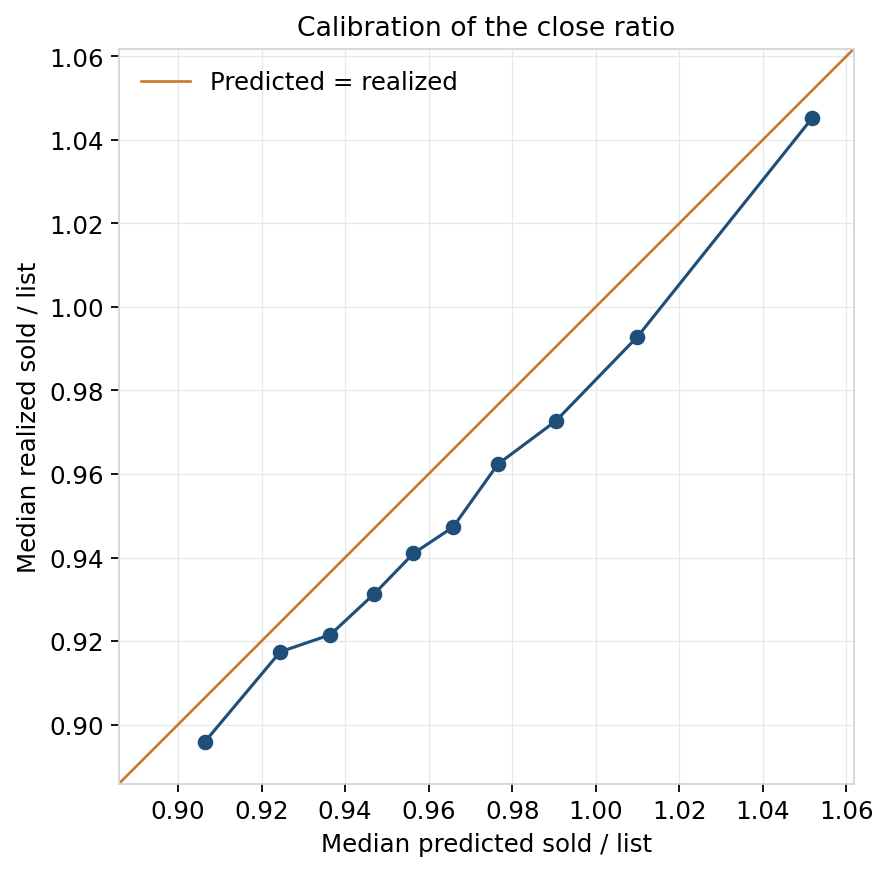
\includegraphics[width=0.48\linewidth]{calibration_ratio.png}\hfill
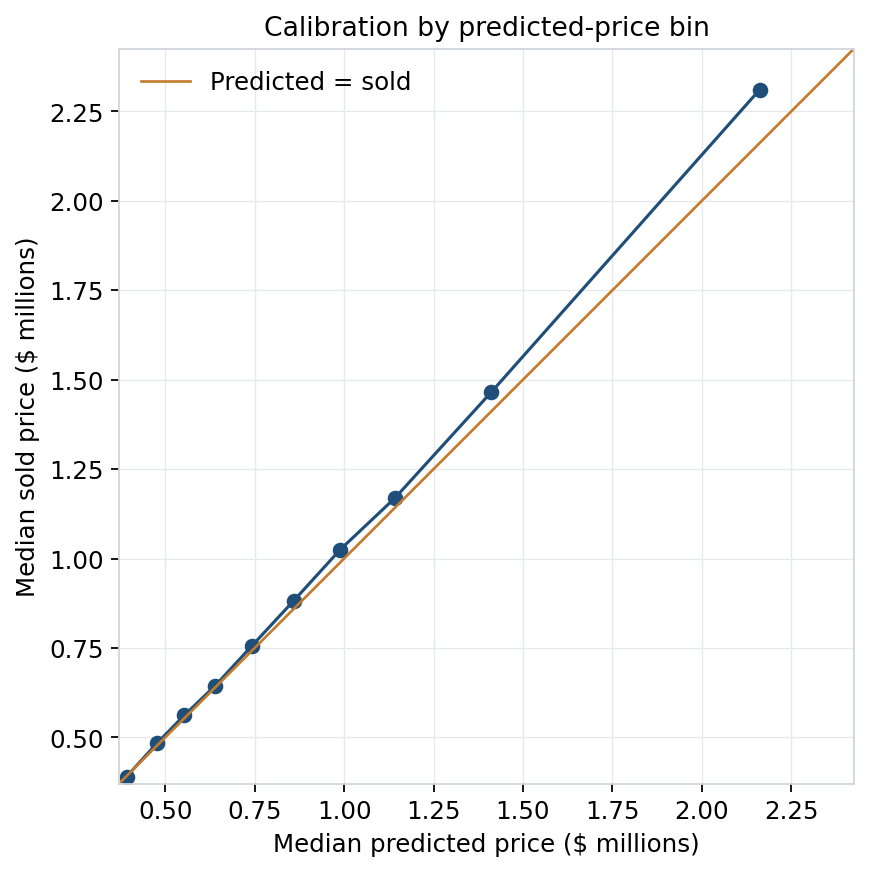
\includegraphics[width=0.48\linewidth]{om_calibration.png}
\caption{Left, \la: median predicted close ratio against median realized close ratio, by bin of predicted ratio. Right, \om: median predicted price against median sold price, by bin of predicted price. Both are the developmental validation, after each model's own calibration.}
\label{fig:cal}
\end{figure}

Through the middle of the book both models order prices correctly. The failure is in the tails, and the tails point in different directions. Section~\ref{sec:fails} is that comparison.

\FloatBarrier
\section{Architecture}
\label{sec:architecture}

The two models share a front door and then fork. Lookups and two small fitted models produce columns. They do not produce a price that we then average. On the list-aware path the fitted upstream piece is a log-linear regression of log sold price on log ask and the attributes. We take its monthly mean residual and forecast that series with a SARIMAX. The forecast is one column, \texttt{list\_month\_factor}. On the off-market path the thirteen phrase flags are patterns we wrote down, so they are not a fitted model. The remarks score is: a ridge of log sold price on a bag of words, fit out of time so a training row is scored by a ridge that has not seen it. The only second stage in either model is the off-market shift \(\delta\).

\begin{figure}[ht]
\centering
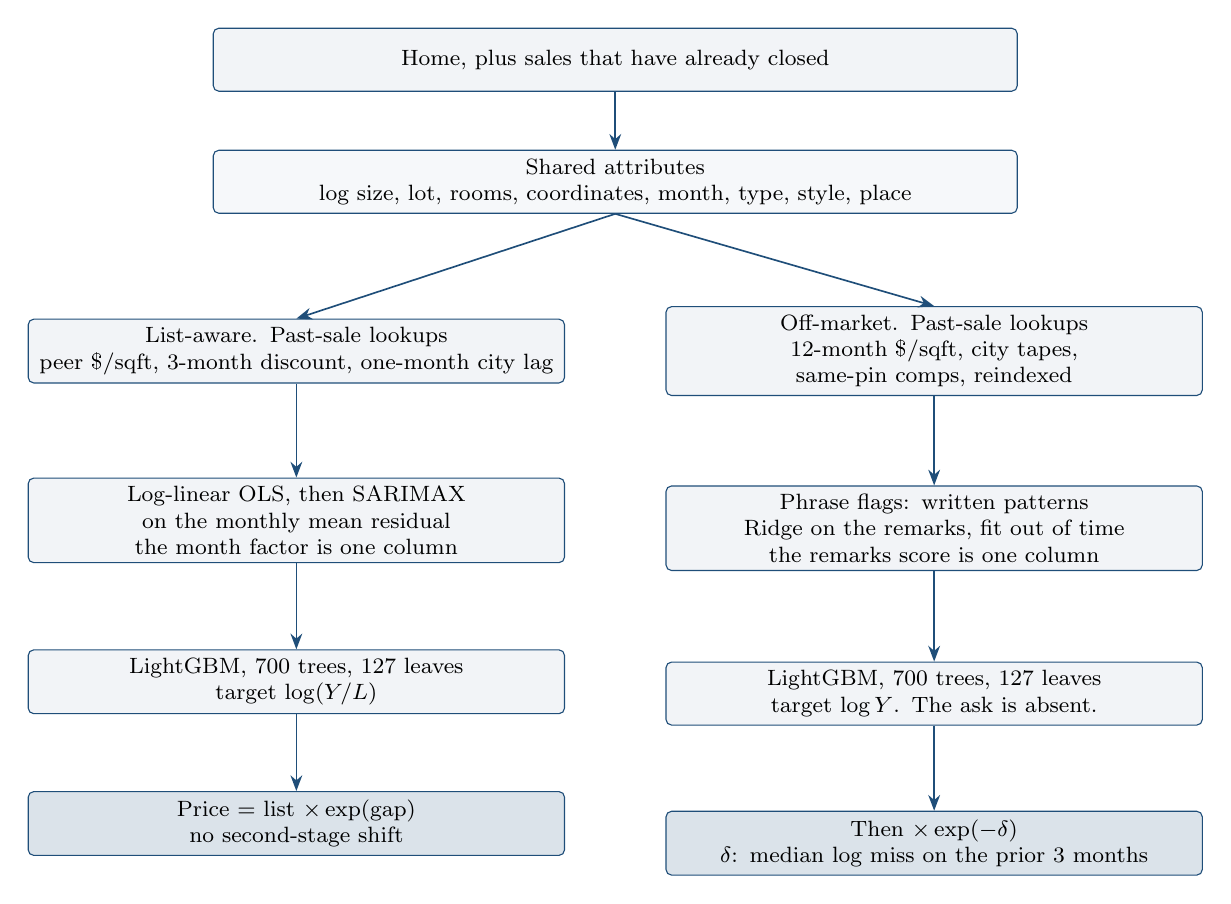
\begin{tikzpicture}[
  font=\footnotesize,
  box/.style={draw=navy, rounded corners=2pt, align=center, inner sep=3pt,
              minimum height=8mm, fill=navy!6, text width=6.6cm},
  arr/.style={-{Stealth[length=2mm]}, semithick, draw=navy}
]
\node[box, text width=10cm] (raw) at (0,0)
  {Home, plus sales that have already closed};
\node[box, text width=10cm, fill=navy!4] (shared) at (0,-1.55)
  {Shared attributes\\ log size, lot, rooms, coordinates, month, type, style, place};
\node[box] (latbl) at (-4.05,-3.7)
  {List-aware. Past-sale lookups\\ peer \$/sqft, 3-month discount, one-month city lag};
\node[box] (lasar) at (-4.05,-5.85)
  {Log-linear OLS, then SARIMAX\\ on the monthly mean residual\\ the month factor is one column};
\node[box] (lgb) at (-4.05,-7.9)
  {LightGBM, 700 trees, 127 leaves\\ target \(\log(Y/L)\)};
\node[box, fill=navy!16] (out) at (-4.05,-9.7)
  {Price \(=\) list \(\times\exp(\mathrm{gap})\)\\ no second-stage shift};
\node[box] (omtbl) at (4.05,-3.7)
  {Off-market. Past-sale lookups\\ 12-month \$/sqft, city tapes,\\ same-pin comps, reindexed};
\node[box] (omtxt) at (4.05,-5.95)
  {Phrase flags: written patterns\\ Ridge on the remarks, fit out of time\\ the remarks score is one column};
\node[box] (lgb2) at (4.05,-8.05)
  {LightGBM, 700 trees, 127 leaves\\ target \(\log Y\). The ask is absent.};
\node[box, fill=navy!16] (out2) at (4.05,-9.95)
  {Then \(\times\exp(-\delta)\)\\ \(\delta\): median log miss on the prior 3 months};
\draw[arr] (raw) -- (shared);
\draw[arr] (shared.south) -- (latbl.north);
\draw[arr] (shared.south) -- (omtbl.north);
\draw[arr] (latbl) -- (lasar);
\draw[arr] (lasar) -- (lgb);
\draw[arr] (lgb) -- (out);
\draw[arr] (omtbl) -- (omtxt);
\draw[arr] (omtxt) -- (lgb2);
\draw[arr] (lgb2) -- (out2);
\end{tikzpicture}
\caption{Scoring path. Shared attributes feed both trees. On the left, lookups and a SARIMAX build columns, and the tree returns a gap around the ask. On the right, lookups, written phrase flags, and a ridge build columns, the tree returns a log price, and one shift scales it. The OLS, the SARIMAX, the ridge, the tables, and \(\delta\) are all fit on sales that closed before the origin. The right path never reads list price, and a building comp has to have closed before the home was listed.}
\label{fig:flow}
\end{figure}

\texttt{make\_model} returns \texttt{ListAwareModel} for the list-aware track and \texttt{OffMarketModel} for the off-market track. The two starter baselines remain in \texttt{models.py}, and \texttt{run.py} leaves them unused.

\FloatBarrier
\section{How we validated}
\label{sec:walk}

A single origin answers ``what if we had stopped in November and predicted the next half year in one shot?'' The claim answers a narrower question. For each sale month \(m\) from December 2025 through May 2026:

\begin{enumerate}
\item The past is every sale with \texttt{date\_sold} strictly before the first day of \(m\).
\item Every table, every category level, every text fit, and the tree are rebuilt on that past. For \om, \(\delta\) is re-estimated on the three months before \(m\).
\item Month \(m\) is scored. Its sold prices are not in any table and not in the tree. On the off-market track the list price is hidden as well.
\item The six months are concatenated. Pooled MdAPE weights homes equally. May, with \(2{,}291\) sales, weighs more than January, with \(1{,}058\).
\end{enumerate}

A building comp inside that refit still has to predate the home's listing. The July--November choices stay fixed. They are not re-searched inside the walk. A random \(k\)-fold split is not a substitute. It leaks later sales into the peer medians, the community leaves, and the building comps.

\texttt{run.py validate} is this procedure for both adopted models. The figure scripts refit the one-origin developmental models and matched the notebooks. They did not repeat the six walk-forward refits. The file \texttt{outputs/validation\_predictions.csv} matches the month tables below, pooled and by month.

\FloatBarrier
\section{Results}
\label{sec:results}

\begin{center}
\small
\begin{tabular}{lrrrr}
\toprule
Model & Homes & MdAPE & MAPE & Median signed \\
\midrule
Handout simple baseline, both tracks & --- & 17.7 & 22.0 & --- \\
Handout ten nearest sales, off-market & --- & 20.8 & 27.4 & --- \\
List price, our refit on these sales & 10{,}069 & 7.26 & 8.09 & \(+5.68\) \\
\la, walk-forward & 10{,}069 & 4.28 & 5.37 & \(+0.90\) \\
12-month community \$/sqft, off-market & 10{,}069 & 15.33 & 20.32 & \(+3.19\) \\
\om, walk-forward & 10{,}069 & 7.45 & 9.79 & \(-0.37\) \\
\bottomrule
\end{tabular}
\end{center}

The home-level bootstrap 95\% intervals from \texttt{run.py report} are \(4.20\)--\(4.39\) on the list-aware MdAPE and \(7.29\)--\(7.63\) on the off-market MdAPE. Homes in one month move together, so the real uncertainty is wider than that.

\begin{center}
\small
\begin{tabular}{l r rr rr}
\toprule
 & & \multicolumn{2}{c}{\la} & \multicolumn{2}{c}{\om} \\
\cmidrule(lr){3-4} \cmidrule(lr){5-6}
Month & Homes & MdAPE & Signed & MdAPE & Signed \\
\midrule
2025-12 & 1{,}238 & 3.97 & \(+1.31\) & 7.42 & \(+0.63\) \\
2026-01 & 1{,}058 & 4.16 & \(+1.33\) & 7.27 & \(-2.50\) \\
2026-02 & 1{,}442 & 4.38 & \(+0.20\) & 8.17 & \(-4.44\) \\
2026-03 & 1{,}816 & 4.14 & \(+0.46\) & 7.10 & \(-1.15\) \\
2026-04 & 2{,}224 & 4.37 & \(+1.31\) & 7.44 & \(+1.65\) \\
2026-05 & 2{,}291 & 4.55 & \(+0.92\) & 7.39 & \(+0.98\) \\
\midrule
Pooled & 10{,}069 & 4.28 & \(+0.90\) & 7.45 & \(-0.37\) \\
\bottomrule
\end{tabular}
\end{center}

The list-aware model beats the ask in every month. Its MdAPE stays inside \(3.97\) to \(4.55\), and its signed error stays positive. The same specification without community as a category has pooled MdAPE \(4.36\). Adding community is ahead in every month. The margin is small, and it is why that category stayed.

The off-market model beats the 12-month anchor by about eight points. The challenger prices the home as that anchor times a tree, and its pooled MdAPE is \(7.50\). The direct model is ahead in five months. February is the exception: the direct model has MdAPE \(8.17\) against the gap model's \(7.86\), and it is \(4.44\%\) low. We kept the direct model because it won the pre-December screen and then held the out-of-time test, not because \(0.05\) points is a large economic gap.

One-origin developmental scores, for the segmented charts in the next section, are \la{} \(4.43\) / \(5.53\) / \(+1.49\) and \om{} \(7.53\) / \(9.77\) / \(-2.10\). Walking forward helps \la{} a little, mostly on the bias, because the discount tables see the latest closes. It barely moves \om's MdAPE, and it moves the bias from \(-2.10\%\) to \(-0.37\%\) because \(\delta\) is refreshed every month.

\begin{figure}[ht]
\centering
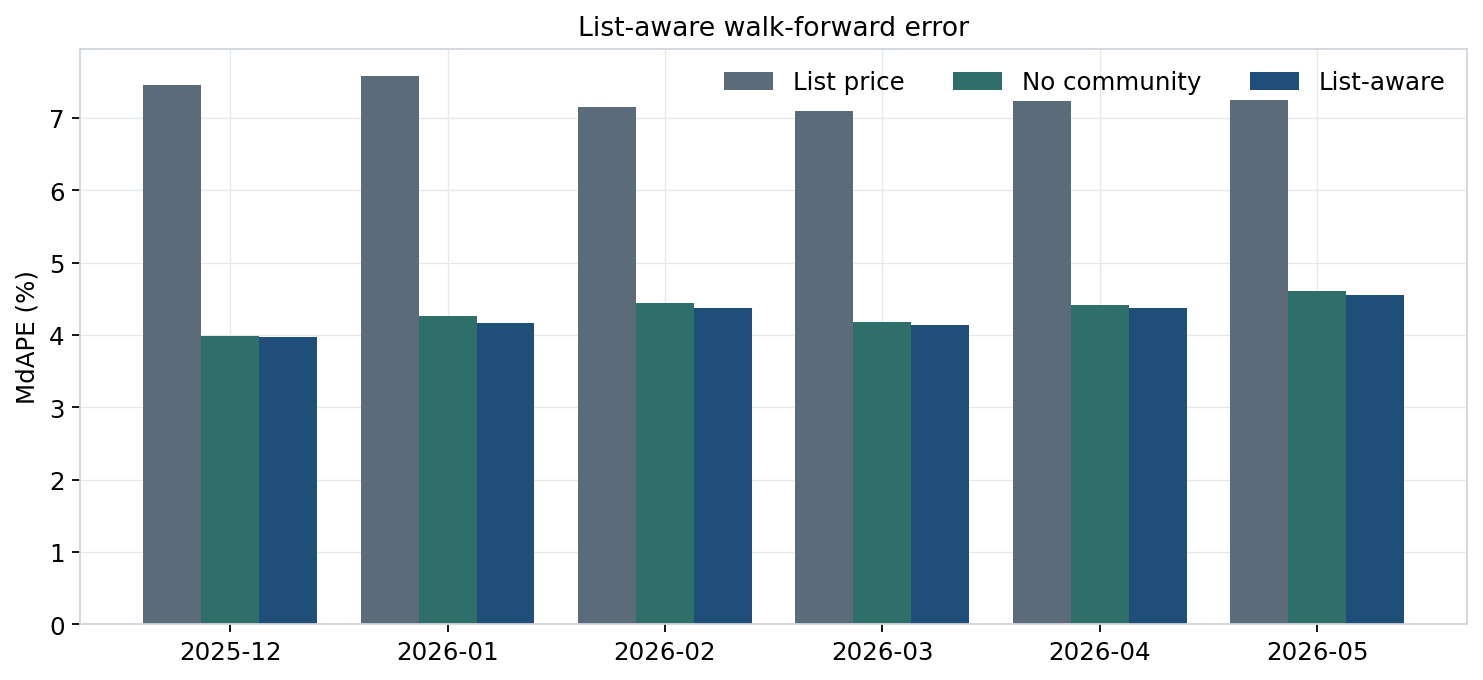
\includegraphics[width=0.49\linewidth]{report_la_mdape.png}\hfill
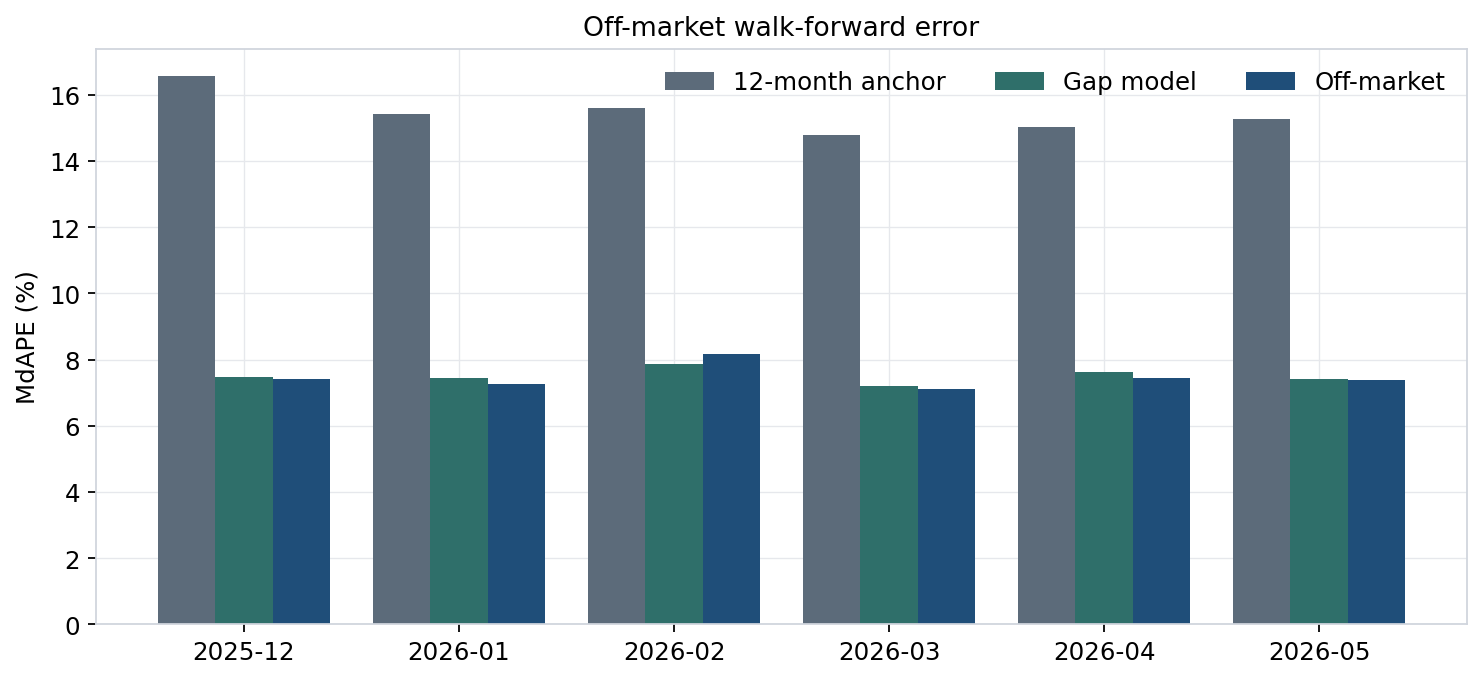
\includegraphics[width=0.49\linewidth]{report_om_mdape.png}
\caption{Walk-forward MdAPE by month. Left, the list price, the list-aware model without community as a category, and the list-aware model. Right, the 12-month community anchor, the gap model, and the off-market model.}
\label{fig:wf}
\end{figure}

\begin{figure}[ht]
\centering
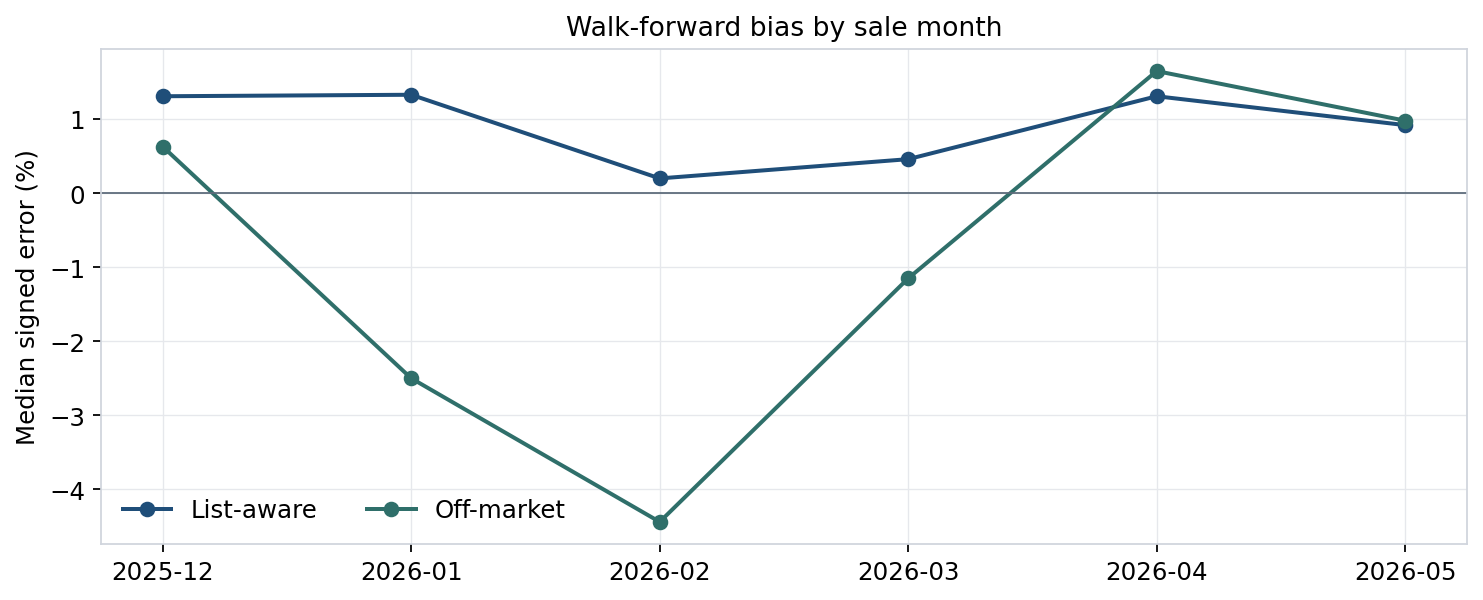
\includegraphics[width=0.92\linewidth]{report_signed.png}
\caption{Median signed error by sale month. Positive means the prediction is high. The list-aware model stays above zero. The off-market model changes sign, and February is the low month.}
\label{fig:signed}
\end{figure}

\FloatBarrier
\section{Where the model fails}
\label{sec:fails}

Segmented errors are from the developmental refit, one origin. They describe where that fit misses. They are not a second walk-forward. The two models fail in different places, and the difference is the ask.

\subsection{By price}

\begin{center}
\small
\begin{tabular}{l rr rr}
\toprule
 & \multicolumn{2}{c}{\la} & \multicolumn{2}{c}{\om} \\
\cmidrule(lr){2-3} \cmidrule(lr){4-5}
Decile (sold price) & MdAPE & Signed & MdAPE & Signed \\
\midrule
D1, \$226k--\$440k & 4.59 & \(+3.69\) & 5.40 & \(+2.53\) \\
D2, \$441k--\$521k & 3.75 & \(+2.07\) & 5.33 & \(-0.50\) \\
D3, \$521k--\$597k & 3.73 & \(+1.87\) & 6.07 & \(-0.78\) \\
D4, \$597k--\$692k & 3.83 & \(+1.56\) & 6.36 & \(-1.31\) \\
D5, \$692k--\$805k & 4.00 & \(+1.45\) & 7.19 & \(-0.08\) \\
D6, \$805k--\$939k & 4.82 & \(+1.16\) & 7.71 & \(-1.63\) \\
D7, \$939k--\$1.10M & 4.72 & \(+1.09\) & 7.84 & \(-2.76\) \\
D8, \$1.10M--\$1.32M & 4.60 & \(+0.47\) & 9.88 & \(-5.63\) \\
D9, \$1.32M--\$1.76M & 5.37 & \(-0.28\) & 10.47 & \(-6.71\) \\
D10, \$1.76M--\$17.0M & 5.57 & \(+0.49\) & 13.58 & \(-10.68\) \\
\bottomrule
\end{tabular}
\end{center}

\la{} is sharpest from about \(\$440{,}000\) to \(\$800{,}000\), with MdAPE under \(4\%\). The cheap decile is accurate in the median-absolute sense and biased high by \(3.7\%\). A user marking the bottom of the book to \la{} will be systematically rich. The top decile widens to \(5.57\%\) and is close to unbiased. The 95th percentile of absolute error on this window is \(14.4\%\), against \(18.7\%\) for the list price on the same homes.

\om{} gets worse as the home gets more expensive. The bottom half of the book, under about \(\$800{,}000\), is where it is sharpest. The top decile is a different product: MdAPE \(13.6\%\), and the predictions are about \(11\%\) low. The cheapest decile is biased the other way, \(+2.5\%\). A user marking luxury collateral to \om{} will be systematically cheap. The 90th and 95th percentiles of absolute error are \(20.5\%\) and \(26.5\%\). About one sale in ten is off by more than \(20\%\). The community anchor on the same homes has a 95th percentile of \(56.6\%\), so the model does shorten the tail. It does not make a \(20\%\) miss unusual.

One percent applied to every home cannot repair either pattern. On \la{} it would push the cheap end, which is already high, further high. On \om{} it would push the cheap end, which is already a bit high, further high, in order to lift a top decile that is \(11\%\) low. We did not adopt a decile-specific correction. Fitting one on the validation months would be using the months we are supposed to be scoring.

\begin{figure}[ht]
\centering
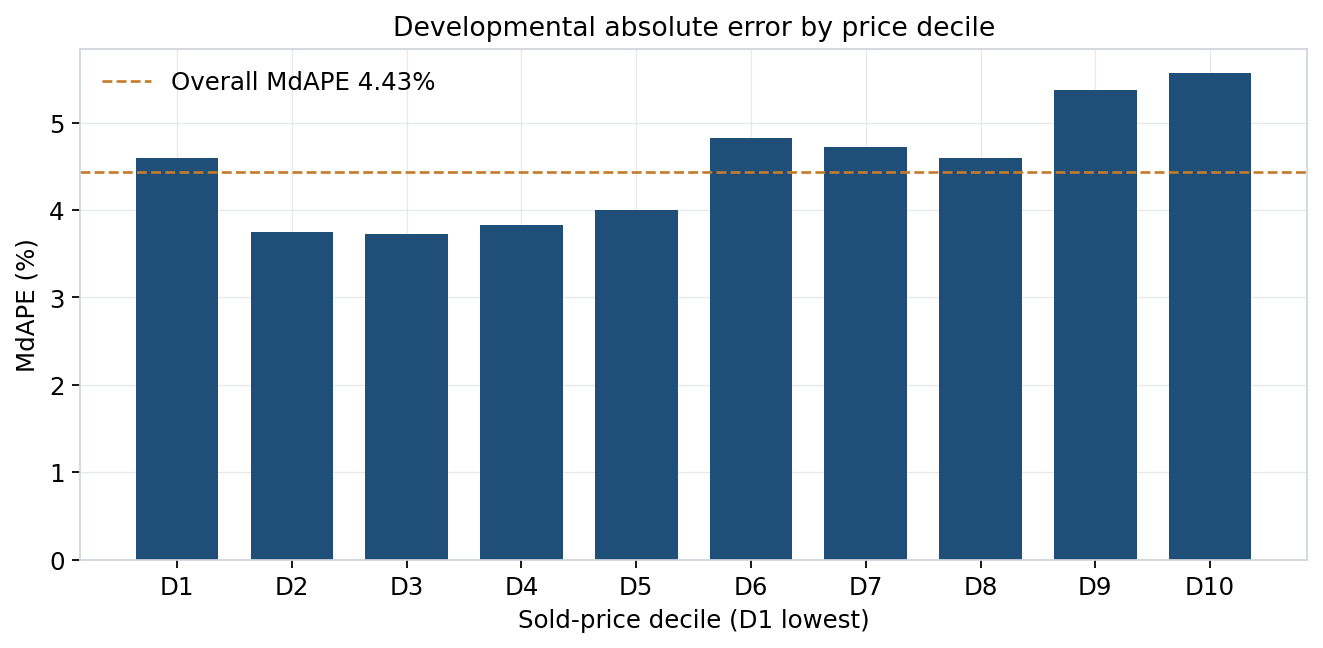
\includegraphics[width=0.49\linewidth]{error_by_decile.png}\hfill
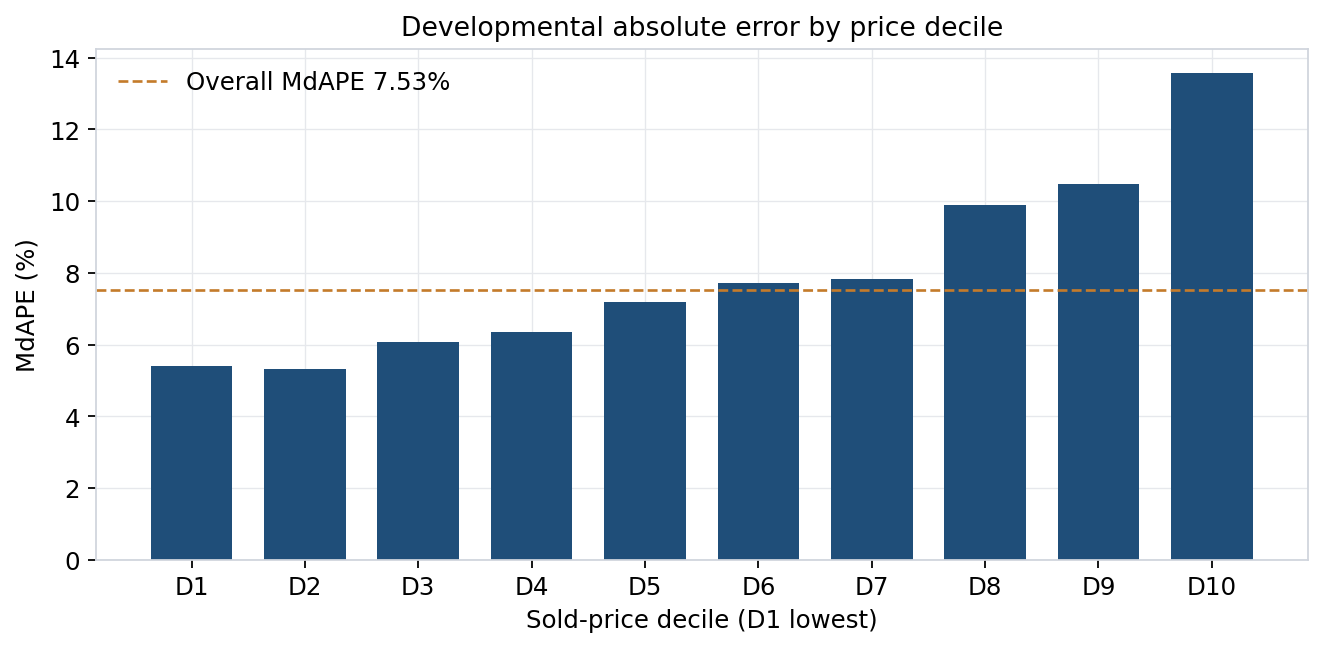
\includegraphics[width=0.49\linewidth]{om_error_by_decile.png}
\caption{Developmental MdAPE by sold-price decile. Left, \la, dashed line \(4.43\%\). Right, \om, dashed line \(7.53\%\).}
\label{fig:decile}
\end{figure}

\subsection{By property type}

\begin{center}
\small
\begin{tabular}{l r rr rr}
\toprule
 & & \multicolumn{2}{c}{\la} & \multicolumn{2}{c}{\om} \\
\cmidrule(lr){3-4} \cmidrule(lr){5-6}
Type & Homes & MdAPE & Signed & MdAPE & Signed \\
\midrule
Condo apartment & 4{,}843 & 3.69 & \(+1.65\) & 6.24 & \(-1.54\) \\
Condo townhouse & 616 & 4.43 & \(+1.45\) & 5.98 & \(-1.42\) \\
Detached & 3{,}123 & 5.52 & \(+1.63\) & 9.60 & \(-2.33\) \\
Semi-detached & 1{,}034 & 5.78 & \(-0.01\) & 9.84 & \(-4.34\) \\
Freehold townhouse & 405 & 5.58 & \(+0.99\) & 9.19 & \(-5.14\) \\
Co-op apartment & 48 & 5.47 & \(+3.60\) & 10.67 & \(-1.47\) \\
\bottomrule
\end{tabular}
\end{center}

Condo apartments are half the validation book and carry both headlines. Ground-oriented homes cost about two extra points of MdAPE on \la{} and about three to four extra points on \om. The off-market gap is the easier one to explain. Same-pin comps exist for \(60\%\) of validation homes, and that coverage is higher where many sales share a coordinate, which is the condo stock. Houses more often have an empty pin and have to be priced from the community tape and the lot. On \la{} the ask already prices the house, and the extra error is what the remarks do not say: two detached houses with the same ask, size, and community can differ by a renovation the model cannot see. Co-op results rest on 48 sales and should not be quoted as a type-level figure.

Municipalities do not separate on either track. \la{} runs from \(4.24\%\) in York (\(n=124\)) to \(4.62\%\) in Scarborough (\(n=1{,}430\)). \om{} runs from \(6.32\%\) in York to \(7.68\%\) in Toronto (\(n=5{,}746\)). The failure mode is price and structure, not the five-way municipal split. That matches the gain shares: community matters, municipality does not.

\subsection{By month, and by a stale tape}

The list-aware model's signed error stays positive in every month, from \(+0.20\%\) in February to \(+1.33\%\) in January (Figure~\ref{fig:signed}). The level is stable and a bit rich. The off-market model's signed error changes sign. It runs from \(-4.44\%\) in February to \(+1.65\%\) in April. The pooled \(-0.37\%\) is a half-year average. A user who marks one month to the off-market model can be several percent off when the half-year pool looks calm.

The off-market model also fails when the comps go stale. Scoring May 2026 with sales cut off at the end of January moves MdAPE from \(7.39\%\) to \(8.38\%\) and the median signed error from \(+0.98\%\) to \(-5.29\%\). A delayed tape makes the model cheap. The off-market test file lists homes from August 2025 through September 2026, so the age of the last sale in the tables is part of the operating design. \la{} is less exposed to the same cut, because the ask is observed on the day we score and already contains the seller's reading of the market. Its remaining exposure is the peer and discount tables, which walk-forward rebuilds every month.

\subsection{Where a feature is simply missing}

\begin{center}
\small
\begin{tabular}{p{4.4cm}p{4.8cm}p{5.0cm}}
\toprule
Gap & How often, developmental validation & What the model falls back on \\
\midrule
\la, three-month community discount & Missing on \(46\%\) of rows. Community cell on \(15\%\). & The type-level three-month median, then the community category and the citywide month factor. \\
\om, same-pin sale & No eligible earlier sale on \(40\%\) of rows. & Community and city dollars per square foot, and size. LightGBM splits on the missing building price. \\
\om, thin community cell & Type or city fallback on \(24\%\) of rows. & The type median if it has 30 sales, otherwise the city. \\
Either model, unseen category & \(0\%\) of communities in this developmental split. & A missing level. We do not borrow a neighbour's label. \\
\bottomrule
\end{tabular}
\end{center}

\section{Limitations}
\label{sec:limits}

\begin{center}
\small
\begin{tabular}{p{3.3cm}p{5.5cm}p{5.6cm}}
\toprule
Limit & \la & \om \\
\midrule
The book & Synthetic. Coordinates must not be joined to maps. A method that works here is evidence about this generating process. & The same. \\
The claim window & Stops in May 2026. The test files run to September 2026 and have no labels here. Nothing in this document is a hidden-test score. & The same. \\
The output & A point estimate. The 95th percentile of \(14\%\) describes one window. It is not a band that updates with the home. & A point estimate. The 95th percentile of \(26\%\) is the same kind of description. \\
Bias we will actually see & About \(+0.9\%\) in every month, and about \(+3.7\%\) on the cheapest decile. An automatic haircut was tested and rejected because it was unstable. & The pool is near zero. February is \(4.4\%\) low. The top decile of the one-shot fit is about \(11\%\) low. \\
A feature that is often empty & The three-month local discount, missing on about half of a frozen November fit. & A same-pin sale, missing on about \(40\%\). A new subdivision is in that half. \\
Text & Left out. It did not move the error. Renovation quality on houses is a credible source of the extra house error. & Kept, and small. The remarks score is \(0.7\%\) of gain. Phrase flags are smaller. The comps are doing the work. \\
Stale information & The ask is current. The peer tables are only as fresh as the last closed sale. & Three stale months cost about one point of MdAPE on May and push the median about \(5\%\) low. \\
Uncertainty & We do not report a home-level interval. The month path is the stability we will stand behind: MdAPE inside a \(0.6\)-point band, bias always positive. & MdAPE inside \(7.10\%\) to \(8.17\%\). The bias is not inside a tight band. \\
\bottomrule
\end{tabular}
\end{center}

The runnable implementations are \texttt{ListAwareModel} and \texttt{OffMarketModel}, called from \texttt{run.py}. A sign-off on this document covers those entry points together with the specification and the evidence. It does not cover a separate production service.

\section{Reproducing the results}
\label{sec:repro}

From the repository root, after \texttt{pip install -r requirements.txt}:

\begin{quote}
\texttt{py -3 run.py validate}\\
\texttt{py -3 run.py report}\\
\texttt{py -3 run.py predict}\\
\texttt{py -3 run.py check}
\end{quote}

\texttt{data.py} loads the files from Hugging Face, dataset \texttt{Baliyang/SSU\_data\_dash}, or from \texttt{DATA\_DIR} when that folder is set. \texttt{validate} is the walk-forward in Section~\ref{sec:walk}. It writes \texttt{validation\_predictions.csv} under \texttt{outputs/}, with prices rounded to the nearest dollar. \texttt{report} writes the score table, the markdown report, and the error-by-price figure. \texttt{predict} is a different fit. It trains on every closed sale through May 2026, so the off-market shift is measured on March--May 2026, and writes the two submission files under \texttt{submissions/}. \texttt{check} confirms one positive finite price per test id.

Columns that can be read off the home are built in \texttt{features.py}. Comp columns, the SARIMAX factor, the remarks ridge, and \(\delta\) are built inside \texttt{fit}, from the sales that fit was given. A training slice under \(8{,}000\) rows, which is only the unit test, uses a short tree. Every fit behind the numbers here is above that cutoff and uses 700 trees. LightGBM \(4.6.0\) is the pin in \texttt{requirements.txt}.

The charts that are not the harness figure come from the figure scripts in \texttt{model-report/}. On 6 and 7 November 2026 those one-origin refits matched the notebooks: list-aware \(4.43\) / \(5.53\) / \(+1.49\), and off-market \(7.53\) / \(9.77\) / \(-2.10\) with a shift of \(+1.58\%\). The walk-forward bars and the signed-error path use the stored month scores, not a new fit.

\appendix
\section{Monitoring rules}
\label{app:monitor}

These are review triggers, not a trading rule. They sit outside the path this window actually produced. A breach is a reason to look, not an automatic switch of model.

\begin{center}
\small
\begin{tabular}{p{3.4cm}p{5.6cm}p{5.4cm}}
\toprule
Measure & Review \la{} if & Review \om{} if \\
\midrule
Monthly MdAPE & Above \(6\%\). The path here is \(4.0\)--\(4.6\). & Above \(10\%\). The path here is \(7.1\)--\(8.2\). \\
Monthly signed error & Outside \(\pm 2.5\%\), or positive and rising for three months. & Outside \(\pm 5\%\). February already reached \(-4.4\%\). \\
A price band & Signed error above \(+5\%\) on sales under \(\$500{,}000\). & Signed error below \(-12\%\) on sales over \(\$1.5\) million. \\
A feature going empty & Community three-month cell on under \(10\%\) of new listings. & An eligible same-pin sale on under \(40\%\) of new homes. \\
The tape & --- & Last sale in the tables more than 90 days before the scoring date. \\
The book & Condo share or median ask moves by more than 10 percentage points. & Condo share moves by more than 10 percentage points. \\
\bottomrule
\end{tabular}
\end{center}

Each score should be stored with the listing identifier, the predicted price, which model produced it, and the month the tables were built through. The list-aware row should also store the list price. The off-market row should store whether a same-pin comp was found. The fail-safe quote on the list-aware track is the ask itself. The close challenger is the same model without community as a category. The fail-safe on the off-market track is the 12-month community anchor when the tree cannot be run, and the gap model when a rolling six-month MdAPE stops favouring the direct model.

\section{List-aware specifications we compared}
\label{app:ladder-la}

Every row is one fit on sales closed before December 2025, scored on December 2025--May 2026. Lower MdAPE is better. A positive signed error means the prediction is high. Adoption used the walk-forward, not the smallest cell in this list. The recent level shift wins this list and loses the walk.

\begin{center}
\small
\begin{tabular}{p{9.4cm}rrr}
\toprule
Specification & MdAPE & MAPE & Signed \\
\midrule
List price & 7.26 & 8.09 & \(+5.68\) \\
OLS, untransformed & 6.86 & 7.83 & \(+5.60\) \\
OLS, log scale & 7.13 & 8.05 & \(+5.95\) \\
Log OLS \(+\) residual forecast & 4.78 & 5.97 & \(+0.25\) \\
Log OLS \(+\) 2022 pulse and level shift & 4.80 & 5.98 & \(+0.41\) \\
Boosted trees, numeric & 4.83 & 5.97 & \(+1.43\) \\
Boosted trees, numeric \(+\) remarks & 4.85 & 5.98 & \(+1.66\) \\
XGBoost, plus peer ask & 4.53 & 5.73 & \(+1.27\) \\
LightGBM, 127 leaves, learning rate 0.03, 700 trees & 4.54 & 5.73 & \(+1.40\) \\
That tree, plus the listing-month factor & 4.51 & 5.68 & \(+1.16\) \\
A recent level shift on that tree & 4.40 & 5.55 & \(-1.11\) \\
Recent community discount, on the log gap & 4.47 & 5.59 & \(+1.07\) \\
List-aware model, community added to that design & 4.43 & 5.53 & \(+1.49\) \\
\bottomrule
\end{tabular}
\end{center}

The longer ladder, including the coordinate experiments and a retuned XGBoost that lost to an untuned one, is in the list-aware track document. One warning sits outside this short list. Retuning depth, learning rate, and tree count on July--November, then refitting, produced a December--May MdAPE of \(4.57\%\), worse than the untuned peer-ask model at \(4.53\%\). A search that wins on the inner slice can lose on the next half year. That is why the final choice was confirmed under walk-forward.

\section{Off-market specifications we compared}
\label{app:ladder-om}

Same origin, same window. The gap model and the specification that added a land term and a drifting forecast tie, because those extras were turned off.

\begin{center}
\small
\begin{tabular}{p{9.6cm}rrr}
\toprule
Specification & MdAPE & MAPE & Signed \\
\midrule
OLS, raw dollars & 21.76 & 29.54 & \(+14.16\) \\
OLS, log price & 20.26 & 27.14 & \(+11.88\) \\
XGBoost on attributes only & 17.28 & 21.17 & \(+14.00\) \\
All-history community \$/sqft & 17.07 & 22.23 & \(+10.84\) \\
12-month community \$/sqft & 15.60 & 20.80 & \(+3.71\) \\
That anchor, plus a level shift & 15.22 & 19.40 & \(-3.22\) \\
LightGBM on the gap around that anchor & 9.40 & 12.13 & \(+1.03\) \\
Extra remarks, full shift & 8.85 & 11.09 & \(-0.76\) \\
Median loss, full shift & 7.70 & 10.14 & \(-2.23\) \\
Gap model, one same-pin sale, full shift & 7.54 & 9.95 & \(-1.72\) \\
Off-market model, direct log price, remarks score, full shift & 7.53 & 9.77 & \(-2.10\) \\
\bottomrule
\end{tabular}
\end{center}

The all-history anchor at \(17.07\%\) sits next to the handout's \(17.7\%\) simple baseline. Beating the long-window median is easy and is not the result. The result is the distance from the 12-month anchor, and then from the gap model, under a walk-forward that cannot see the scored month. On that walk-forward the order is the same and the margin between the off-market model and the gap model is \(0.05\) points.

\section{References}

\begin{itemize}
\item Friedman, J. (2001). Greedy function approximation: a gradient boosting machine. \emph{Annals of Statistics}, 29(5), 1189--1232.
\item Ke, G., Meng, Q., Finley, T., Wang, T., Chen, W., Ma, W., Ye, Q., and Liu, T.-Y. (2017). LightGBM: a highly efficient gradient boosting decision tree. \emph{Advances in Neural Information Processing Systems}, 30.
\item Rosen, S. (1974). Hedonic prices and implicit markets: product differentiation in pure competition. \emph{Journal of Political Economy}, 82(1), 34--55.
\end{itemize}

The stationarity checks use the augmented Dickey--Fuller and KPSS tests, and a robust STL decomposition with a 12-month period. Walk-forward validation is the procedure in \texttt{handout.md} and \texttt{run.py}: train on the past, score the next month, and repeat. The handout bars cited in Section~\ref{sec:results} were not refit here.

\end{document}
